%
% This is the LaTeX template file for lecture notes for CS294-8,
% Computational Biology for Computer Scientists.  When preparing 
% LaTeX notes for this class, please use this template.
%
% To familiarize yourself with this template, the body contains
% some examples of its use.  Look them over.  Then you can
% run LaTeX on this file.  After you have LaTeXed this file then
% you can look over the result either by printing it out with
% dvips or using xdvi.
%
% This template is based on the template for Prof. Sinclair's CS 270.

\documentclass[twoside, 12pt]{article}
\usepackage{graphics}
\usepackage[margin=6mm]{geometry}




%
% The following commands set up the lecnum (lecture number)
% counter and make various numbering schemes work relative
% to the lecture number.
%
%\newcounter{lecnum}
%\renewcommand{\thepage}{\thelecnum-\arabic{page}}
%\renewcommand{\thesection}{\thelecnum.\arabic{section}}
%\renewcommand{\theequation}{\thelecnum.\arabic{equation}}
%\renewcommand{\thefigure}{\thelecnum.\arabic{figure}}
%\renewcommand{\thetable}{\thelecnum.\arabic{table}}



%
% The following macro is used to generate the header.
%
\newcommand{\lecture}[4]{
%   \pagestyle{myheadings}
%   \thispagestyle{plain}
%   \newpage
%  \setcounter{lecnum}{#1}
%   \setcounter{page}{1}
%   \noindent
%   \begin{center}
%   \framebox{
%      \vbox{\vspace{2mm}
%    \hbox to 6.28in { {\bf UGBA 141 Production and Operations Management
%                        \hfill Spring 2022} }
%       \vspace{4mm}
%       \hbox to 6.28in { {\Large \hfill Reference Sheet : #2 (March 7)  \hfill} }
%       \vspace{2mm}
%       \hbox to 6.28in { {\it 
%       Lecturer: #3 
%       \hfill 
%       GSI: #4} }
%      \vspace{2mm}}
%   }
%   \end{center}
%  \markboth{Lecture #1: #2}{Lecture #1: #2}
%   {\bf Disclaimer}: {\it These notes have not been subjected to the
%   usual scrutiny reserved for formal publications.  They may be distributed
%   outside this class only with the permission of the Instructor.}
 % \vspace*{4mm}
}

%
% Convention for citations is authors' initials followed by the year.
% For example, to cite a paper by Leighton and Maggs you would type
% \cite{LM89}, and to cite a paper by Strassen you would type \cite{S69}.
% (To avoid bibliography problems, for now we redefine the \cite command.)
% Also commands that create a suitable format for the reference list.
\renewcommand{\cite}[1]{[#1]}
\def\beginrefs{\begin{list}%
        {[\arabic{equation}]}{\usecounter{equation}
         \setlength{\leftmargin}{2.0truecm}\setlength{\labelsep}{0.4truecm}%
         \setlength{\labelwidth}{1.6truecm}}}
\def\endrefs{\end{list}}
\def\bibentry#1{\item[\hbox{[#1]}]}

%Use this command for a figure; it puts a figure in wherever you want it.
%usage: \fig{NUMBER}{SPACE-IN-INCHES}{CAPTION}
\newcommand{\fig}[3]{
			\vspace{#2}
			\begin{center}
			Figure \thelecnum.#1:~#3
			\end{center}
	}
% Use these for theorems, lemmas, proofs, etc.
%\newtheorem{theorem}{Theorem}[lecnum]
%\newtheorem{lemma}[theorem]{Lemma}
%\newtheorem{proposition}[theorem]{Proposition}
%\newtheorem{claim}[theorem]{Claim}
%\newtheorem{corollary}[theorem]{Corollary}
%\newtheorem{definition}[theorem]{Definition}
%\newenvironment{proof}{{\bf Proof:}}{\hfill\rule{2mm}{2mm}}


% self added package
\usepackage{amsmath}
 \usepackage{graphicx}
 \usepackage[nodisplayskipstretch]{setspace} % reduce space between equations

% **** IF YOU WANT TO DEFINE ADDITIONAL MACROS FOR YOURSELF, PUT THEM HERE:



\begin{document}
%FILL IN THE RIGHT INFO.
%\lecture{**LECTURE-NUMBER**}{**DATE**}{**LECTURER**}{**SCRIBE**}
%\lecture{1}{Midterm}{Park Sinchaisri}{Hansheng Jiang}
%\footnotetext{These notes are partially based on those of Nigel Mansell.}

% **** YOUR NOTES GO HERE:

% Some general latex examples and examples making use of the
% macros follow.  
%**** IN GENERAL, BE BRIEF. LONG SCRIBE NOTES, NO MATTER HOW WELL WRITTEN,
%**** ARE NEVER READ BY ANYBODY.

\begin{center}
	{\bf \large Spring 2022 UGBA 141 Midterm Reference Sheet}
\end{center}

\begin{enumerate}

\item {\bf Process}
	\[
	\text{Capacity} = \frac{1}{\text{Processing time of $1$ unit}}.
	\]
	\[
\text{ For a single linear process, }	\text{Process capacity} = \text{Minimum} \{ \text{Capacity of resource } 1, \dots, \text{Capacity of resource } n \}.
	\]
	\[
	\text{Flow rate} = \text{Minimum} \{ \text{Available input, Demand, Process capacity} \}.
	\]
		\[
		\text{Utilization} = \frac{\text{Flow rate}}{\text{Capacity}}, 	\text{Implied utilization} = \frac{\text{Demand}}{\text{Capacity}}.
		\]
		\[
		\text{Time to fulfill $X$ units (steady state)} = \frac{X}{\text{Flow rate}} = X \times \text{Cycle time}.
		\]
			\[
		\text{Labor content} = \text{Sum of processing times with labor}, 	\text{Cost of direct labor} = \frac{\text{Total wages}}{\text{Flow rate}}.
		\]
		\[
		\text{Average labor utilization}  = \frac{\text{Labor content $\times$ Flow rate}}{\text{Number of workers}}.
		\]
		\[
		\text{Idle time} = \text{Cycle time} - \text{Processing time of the single worker}.
		\]
		


\item {\bf Quality}
\begin{figure}[!htbp]
		\centering
		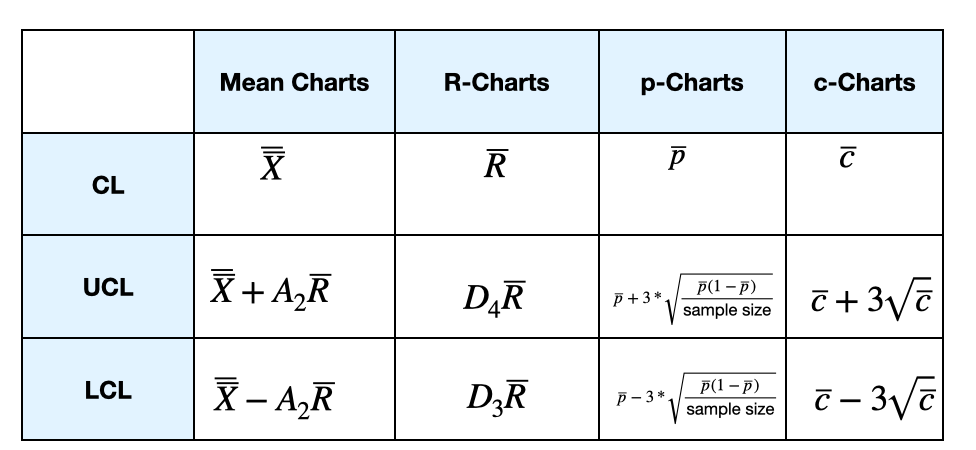
\includegraphics[width = 0.7\textwidth]{control_chart_screenshot}
		\caption{Computation of CL, UCL, LCL for control charts}
	\end{figure}

For centered process , 
		$
		C_p = \frac{\text{USL}-\text{LSL}}{6 \hat{\sigma}}.
		$ For off-centered process, $
		C_{pk} = \min \left\{ \frac{\text{USL} - \overline{X}}{3 \hat{\sigma}},  \frac{\overline{X}-\text{LSL}}{3 \hat{\sigma} } \right\}.
	    $


\item {\bf Inventory}

\begin{enumerate}
	\item Economic Order Quantity (EOQ):
	$
	\text{EOQ} = \sqrt{\frac{2 \times S \times D}{h}},
	$

	\item Continuous review model (Q,R):
	$
	Q =  \sqrt{\frac{2 S D}{h}}, R = \mu_{LT} + z \sigma_{LT}.
	$

	\item Periodic review model (P,T):
    $
	P = \sqrt{ \frac{2S}{Dh}}, T = \mu_{P+LT} + z \sigma_{P+LT}.
	$
	
	\item Newsvendor:
	The order quantity $Q^*$ satisfies
    $
	\text{Prob} (D \leq Q^*) = 	\text{Critical ratio} = \frac{G}{G+L}.
    $
    
    \item Annual inventory turns = Annual cost of goods sold (COGS) \ /  Average inventory (\$).
	
\end{enumerate}



\end{enumerate}














%
%\section*{References}
%\beginrefs
%
%
%\bibentry{TC2006}{\sc C.~Terwiesch} and {\sc G.~Cachon}, 
%  Matching supply with demand: An introduction to operations management (Chapter 2, 5, and14), {McGraw-Hill~2006}
%  
%\bibentry{SG2018}{\sc R.~Schroeder} and {\sc S. M. ~Goldstein}, 
%Operations Management in the Supply Chain (Chapter 14), {McGraw-Hill~2018}
%
%\endrefs


\end{document}





